\PassOptionsToPackage{no-math}{fontspec}%禁用了使用fontspec宏包中的数学字体功能。
\PassOptionsToPackage{AutoFakeBold=true,AutoFakeSlant=true}{xeCJK}%让xeCJK宏包自动产生伪粗体和伪斜体效果。

\documentclass{book}
\usepackage[heading=true
,scheme=chinese%中文方案
,fontset=none%不使用默认的字体设置
,space=auto%自动调整中英文间距
]{ctex}
\setCJKmainfont{FangZhengShuSong-GBK-1.ttf}[Path=/Users/virhuiai/hlProjects/Latex-Typesetting-Hub/font/方正/]%设置文本的中文有衬线字体
\setCJKsansfont{FangZhengHeiTi-GBK-1.ttf}[Path=/Users/virhuiai/hlProjects/Latex-Typesetting-Hub/font/方正/]%设置文本的中文无衬线字体为
\setCJKmonofont{FangZhengFangSong-GBK-1.ttf}[Path=/Users/virhuiai/hlProjects/Latex-Typesetting-Hub/font/方正/] %设置文本的中文等宽字体 

\usepackage[all]{tcolorbox}
\usepackage{paralist}
\begin{document}

% 定义打开和关闭设置临时计数器命令的功能
\newcommand\counterSetTmpOpen{\providecommand{\counterSetTmp}{}\renewcommand\counterSetTmp[2]{\setcounter{##1}{##2}}}
\newcommand\counterSetTmpClose{\providecommand{\counterSetTmp}{}\renewcommand\counterSetTmp[2]{}}
\counterSetTmpOpen
% \counterSetTmpClose

\newcounter{Emp}[chapter]
\renewcommand{\theEmp}{\thechapter.\arabic{Emp}}
\newcommand{\EX}{\par%
{\bf 例~}%
\refstepcounter{Emp}{\bf\theEmp}\hspace{1em}}

% \counterSetTmp{chapter}{6}%第7章ok v5
\chapter{列表}%-v5

列表就是将某一论述的内容分成若干个简短的条目,并按一定的顺序排列,以达到{\bf 简明扼要,醒目直观}的阅读效果。列表是论文写作的重要论述手段。

\LaTeX{\tiny 提供}%有3种
的标准列表环境:
\begin{compactitem}
  \item
  常规列表环境{itemize}%,{[ˈaɪtəmaɪz]逐条列记}
\item
  排序列表环境{enumerate}%,{[ɪˈnjuːməreɪt]列举}%[ɪ'njuːməreɪt] [美: ɪ'numəret] [英: ɪ'njuːməreɪt]
\item
  解说列表环境{description}%,{[dɪˈskrɪpʃn]描述}
\end{compactitem}

可使用相关的命令在全文或者局部文本中修改这3种标准列表环境的排版样式;
 
若调用paralist和mdwlist等列表宏包还可以得到具有更多排版样式的列表环境;

此外,LaTeX还提供有两个通用列表环境:
\begin{compactitem}
\item list
\item trivlist
\end{compactitem}
%latexdef -s 16KTemplateBook02.tex  list
%latexdef -s 16KTemplateBook02.tex trivlist
作者可使用它们自行创建新的列表环境或者其他用途的环境。
% \section{通用列表环境list}

% 前面已经介绍了多种列表环境,可以基本满足论文写作的需要,
如果对某个列表环境的排版样式不够满意而又难以修改,
可采用list通用列表环境,\index{environment}{列表!通用列表!list}%
上述各种列表环境都是用它创建的,其命令结构为:
\begin{minted}{latex}
\begin{list}{默认标号}{声明}
\item[标号] 条目1
\item[标号] 条目2
......
\end{list}
\end{minted}



通用列表环境list之间相互嵌套可多达6层。

\LaTeX 系统提供了一组长度数据命令,专用于修改list通用列表环境中的各种条目尺寸,可统称为条目尺寸命令,它们各自的控制范围如图\ref{fig:条目尺寸命令示意图}所示。

\begin{figure}[htbp]
\centering
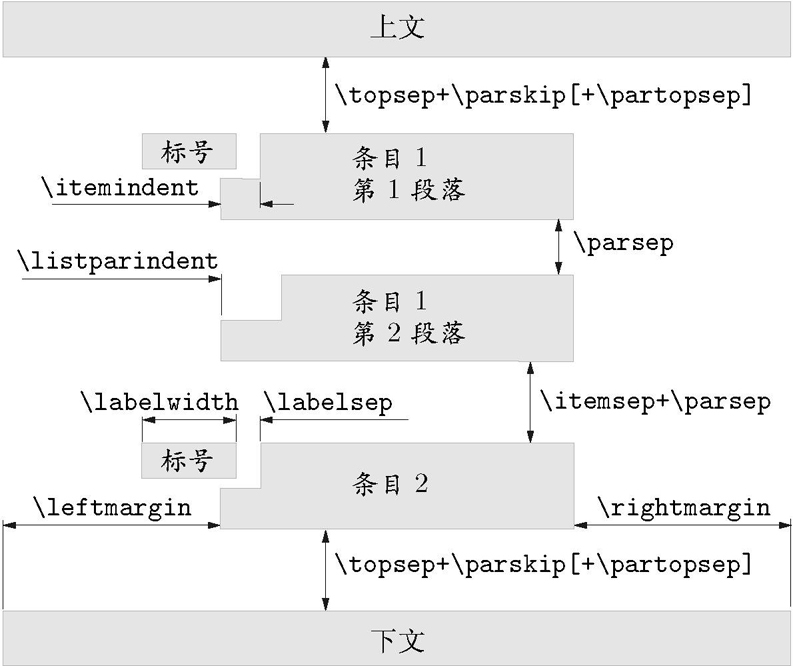
\includegraphics[width=0.5\linewidth]{我的学习笔记_XeLaTeX/列表/通用列表环境_list.png}
\caption{条目尺寸命令示意图}\label{fig:条目尺寸命令示意图}
\end{figure}%% todo tikz 画

% % %\begin{Verbatim}
% % %%垂直方向全部置0
% % %\parsep=0pt
% % %\itemsep=0pt
% % %\topsep=0pt
% % %\partopsep=0pt
% % %\end{Verbatim}

% % %图7.1 \textbf{条目尺寸命令示意图}

% 图\ref{fig:条目尺寸命令示意图}中的各种条目尺寸命令都可在通用列表环境list的声明
% 中,使用长度赋值命令,%例如~\verb|\rightmargin=20pt|~,
% 对其重新赋值。图\ref{fig:条目尺寸命令示意图}中的各种条目尺寸命令及其说明如下。

% % %%%%%%% 长的desc,前后加rule
% % %\noindent\nopagebreak
% % %\rule{\linewidth}{0.1ex}
% % %\nopagebreak
% \begin{description}

% \item [\cs{itemindent}]
% 每个条目的首行缩进宽度,默认值为0pt,可以取负值。%
% %\\此处~\verb|\the\itemindent|~:\the\itemindent%
% %
% \item[\cs{itemsep}]
% 条目之间附加的垂直距离,默认值是~\verb|4.5pt plus 2pt minus 1pt|~。\\
% 条目之间的距离等于~\verb|\itemsep|~加上~\verb|\parsep|~%\\%
% %此处~\verb|\the\itemsep|~:\the\itemsep\\
% %此处~\verb|\the\parsep|~:\the\parsep
% \item[\cs{labelsep}]
% 盛放标号的盒子右端与条目首行文本之间的距离,其默认值为~\verb|2em|,可以取负值。%
% %\\此处~\verb|\the\labelsep|~:\the\labelsep%
% \item[\cs{labelwidth}]
% 盛放标号的盒子名义宽度,默认值为~\verb|2em|~,如标号的自然宽度小于等于此值,标号将在盒内右对齐,否则,盒子的宽度等于标号的自然宽度,这将造成条目首行文本向右缩进。此值必须为正。
% \EX{}%\label{ex:}%
% 重新定义~\verb|\makelabel|~使之左对齐的%2019-08-18 13:37:56
% \begin{Verbatim}
% \renewcommand\makelabel[1]{\texttt{\vSpecColor{##1}}\hfil}
% \end{Verbatim}
% \item[\cs{leftmargin}]
% 条目左缩进宽度,即条自左端与所在环境左端,通常是版心左端之间的%
% 空白宽度,或者是本层条目左端与上层条目左端之间的空白宽度。此%
% 值不能为负,且该值与列表嵌套的层次有关,每层列表的条目左缩%
% 进宽度可分别用命令~\verb|\leftmargini|~、~\verb|\leftmarginii|~、~\verb|\leftmarginiii|~和~\verb|\leftmarginiv|表示,%
% %它们的默认值分别是2.5em、2.2em、1.87em和1.7em,
% 其中第1层的~\verb|\leftmargini|~等于~\verb|\leftmargin|~。
% %\begin{Verbatim}
% %% 如
% %\setlength\leftmargin{\labelwidth+\labelsep}
% %\end{Verbatim}
% %左缩进设置例子
% \item[\cs{listparindent}]
% 每个条目从第二段起每段首行缩进宽度,默认0pt,可设为负值。
% %
% \item[\cs{parsep}]
% 一个条目中的两段落之间附加的垂直空白%.其默认值是~\texttt{4.5pt plus 2pt minus 1pt}。
% %
% \item[\cs{parskip}]
% 列表与上文或下文之间设定的垂直空白,其默认值是~\verb|0pt plus 1pt|~。
% %
% \item[\cs{partopsep}]
% 附加垂直空白,其默认值是~\verb|3pt plus 1pt minus 1pt|~。
% %
% \item[\cs{rightmargin}]
% 条目右缩进宽度.即条目右端与所在环境右端,通常是版心右端之间的空%
% 白宽度.或本层条目右端与上层条目右端之间的空白宽度。此值不能为%
% 负。在标准文类中,条目右缩进宽度的默认值都为~\verb|0pt|。
% %
% \item[\cs{topsep}]
% 列表与上、下文之间设定的垂直空白,默认值~\verb|9pt plus 3pt minus 5pt|~。
% %\\此处~\verb|\the\topsep|~:\the\topsep
% \end{description}

% 在上述条目尺寸命令中,表示水平方向的长度都是刚性的,以保证列表格式的一致性,而表示垂直方向的长度都是弹性的,当使用版心底部对齐命令~\verb|\flushbottom|~时,这些弹性长度将起到伸缩调控的作用。

% 列表与上下文之间的总垂直空白是~\verb|\topsep+\parskip|~,如果列表是以新段落开始,即列表之前是一空行或换段命令,则列表与上下文之间还附加一段~\verb|\partopsep|~垂直空白。

% %\textbf{例7.25}
% \EX{}\label{ex:7.25}%
% 将通用列表环境所生成条目序号的计数形式设置为大写罗马数字。
% \begin{center}
% \includegraphics[width=\linewidth]{ex-7-25}
% \end{center}

% 上例中,首先在列表环境之外,用计数器创建命令新设一个名为Gaus的计数器,然后在声明
% 中用计数器调用命令调用Gaus计数器作为列表的序号计数器;这样,默认标号
% 就可以将Gaus中的数值作为条目的序号。

% %\textbf{例7.26}
% \EX{}\label{ex:7.26}
% 条目的标号默认为右对齐。在例\ref{ex:7.25}中,由于A-Ⅰ与A-Ⅱ的自然宽度不一致,造成列表左边缘参差不齐。可以在声明中将标号定义为左对齐。
% \begin{Verbatim}
% \renewcommand\makelabel[1]{#1\hfil}}
% \end{Verbatim}
% \begin{center}
% \includegraphics[width=\linewidth]{ex-7-26}
% \end{center}

% 条目命令~\verb|\item|~产生的标号是由~\verb|\makelabel|~命令根据默认标号
% 生成的,可使用重新定义命令对~\verb|\makelabel|~重新定义;盛放标号的是左右模式的盒子,左对齐命令~\verb|\raggedright|~在其中并不起作用,只能用~\verb|\hfil |~命令将标号~\verb|#1|~挤到标号盒子的左端;还可以使用粗体命令~\verb|\textbf{#1}|~将标号中的字符变成粗体。

% %\textbf{例7.27}
% \EX{}\label{ex:7.27}
% 常规列表的标志符号都是黑色的,标志符号也不易改换。使用通用列表定义一个标志符号为蓝色,标志符号可变换的常规列表环境。
% \begin{center}
% \includegraphics[width=\linewidth]{ex-7-27}
% \end{center}

% 在上例中,只要改换colorlist环境命令中编号参数的编号,即改换pifont宏包提供的各种符号的编号,就可改换列表的标志符号。

% %\textbf{例7.28}
% \EX{}\label{ex:7.28}
% 在通用列表环境的默认标号
% 参数中,使用ctex中文字体宏包提供的~\verb|\chinese|~中文计数形式命令,就可以将条目序号的计数形式改为中文小写数字。
% \begin{center}
% \includegraphics[width=\linewidth]{ex-7-28}
% \end{center}

% %\textbf{例7.29}
% \EX{}\label{ex:7.29}
% 通用列表环境list机动灵活,变化多端,但须使用的命令颇多,故很少在论文写作中直接使用,它强大的功能主要应用在宏包文件里定义各种用途的环境。本例就是用通用列表环境定义一个新的列表环境Notes。
% \begin{center}
% \includegraphics[width=\linewidth]{ex-7-29}
% \end{center}


% 在上例源文件中,将条目左缩进宽度设为0pt,使条目段落左端与所在环境的左端对齐,并把标号与条目首行之间的距离由默认值的0.5em扩大为1em,同时为了使标号不致凸出环境左端,将条目首行的缩进宽度由默认值的0pt改为3em。

% %\textbf{例7.30}
% \EX{}\label{ex:7.30}
% 可用list环境来修改或创建新的列表环境,如创建一个新的解说列表环境,将其中所有词条左对齐,词条的字体改为倾斜体,所有条目行的左缩进宽度相等。
% \begin{center}
% \includegraphics[width=\linewidth]{ex-7-30}
% \end{center}

% 在上例中,新创建的解说列表环境Description带有一个参数,可将字符最多的词条放入其中,以测定其自然宽度;条目段落的左缩进宽度等于字符最多的词条宽度加词条与条目之间的距离,即~\verb|\labelwidth+\labelsep|~,因为用到加法,还需调用calc算术宏包。

% %\textbf{例7.31}
% \EX{}\label{ex:7.31}
% 在论文写作中经常要用到常规列表,有时总感到条目段落的左缩进宽度或者右缩进宽度不太合适,调整起来很麻烦,需要在成堆的命令里查找适合的命令;条目标志的样式以及条目首行缩进的宽度最好也都能在同一环境中自行设定。为此,可采用通用列表自定义一个带有4个参数的常规列表环境Mylist。
% \begin{center}
% \includegraphics[width=\linewidth]{ex-7-31}
% \end{center}

% 其中的各种参数说明如下。

% \begin{description}
% %{右缩进宽度}
% \item [标志] 可选参数,用于设定条目标志的样式,其默认值设定为~\verb|$\bullet$|~。
% \item [首行缩进] 设置条目段落首行的缩进宽度。
% \item [左缩进宽度] 设置条目段落左端与版心左端之间的水平空白宽度。
% \item [右缩进宽度] 设置条目段落右端与版心右端之间的水平空白宽度。
% \end{description}

% 在上例中,将各种附加的垂直空白宽度都设置为0pt,使所有条目段落的行距与环境之外的文本行距相等。
% \begin{Verbatim}
% \topsep=0pt
% \itemsep=0pt
% \parsep=0pt
% \partopsep=0pt
% \end{Verbatim}
% %\textbf{例7.32}
% \EX{}\label{ex:7.32}
% 通用列表环境list还可以用来创建其他非列表环境,例如创建一个带有上下水平分隔线、具有序号并且外部文本可以引用的推论环境。
% \begin{center}
% \includegraphics[width=\linewidth]{ex-7-32}
% \end{center}

% 上例源文件说明如下。

% \begin{compactitem}
% %[(1)]
% \item 用命令~\verb|\newcounter{Educt}[chapter]|~新建一个计数器,作为推论环境的序号计数器;其中可选参数chapter表示:如果章计数器chapter加1,这个新建的Educt计数器将清零,也就是说该推论环境是以章为排序单位。系统也将随即自动定义一条命令:
% \begin{Verbatim}
% \newcommand{\theEduuct}{\arabic{Educt}}
% \end{Verbatim}

% \item 使用新环境定义命令~\verb|\newenvironment|~定义一个名为Educt的推论环境。

% \item 重新定义当前书签命令~\verb|\@currentlabel|~,使引用格式改为``\textbf{推论}
% 序号'',并将其用计数器命令~\verb|\refstepcounter|~传递给Educt环境中的书签命令~\verb|\label|~。

% \item 在推论的前后用两条醒目的水平实线将其与上下文截然分开,以利于读者查找识别;在线段命令~\verb|\rule|~的前后使用~\verb|\nopagebreak|~命令,以防在此处换页。
% \end{compactitem}





% Clojure

\end{document}
%mypdf 我的学习笔记_XeLaTeX